\documentclass{siamart1116}

\usepackage{amsfonts,amsmath,amssymb}
\usepackage{mathrsfs,mathtools}
\usepackage{enumerate}
\usepackage{hyperref}
\usepackage{esint}
\usepackage{graphicx}
\usepackage{bm}
\usepackage{commath}
\usepackage{esint}
\usepackage{algorithm,algorithmic}
\DeclareMathAlphabet{\mathpzc}{OT1}{pzc}{m}{it}
	
\graphicspath{{/Users/Luke/Desktop/EXTREEMS/Paper/}}	
%%%%%%%%%%%%%%%%%%%%%%%%%%%%%%%%%%
% comment before submission
\usepackage[textsize=small]{todonotes}
\newcommand{\HA}[1]{{\color{red}~\textsf{#1}}}
\newcommand{\LB}[1]{{\color{blue}~\textsf{#1}}}
\usepackage[notref,notcite]{showkeys}
%%%%%%%%%%%%%%%%%%%%%%%%%%%%%%%%%%


\title{Fractional Dynamics for Quantum Random Walks\thanks{The work of the first author is partially supported by NSF grant DMS-1521590. The work of second author is partially supported by NSF grant DMS-1407087.}}
\author{Harbir Antil\thanks{Department of Mathematical Sciences, George Mason University, Fairfax, VA 22030, USA. \texttt{hantil@gmu.edu}}
\and 
Lucas Bouck\thanks{Department of Mathematical Sciences, George Mason University, Fairfax, VA 22030, USA. \texttt{lbouck@gmu.edu}}
}
%\date{\today}							% Activate to display a given date or no date

\pagestyle{myheadings}
\thispagestyle{plain}
\markboth{H.~Antil, L.~Bouck}{Fractional Dynamics for Quantum Random Walks}


\begin{document}

\maketitle

\begin{abstract}
Quantum random walks (QRWs) are important tools for the development of algorithms in the growing field of quantum computing. The standard partial differential equation (PDE) based models of QRWs fail to capture the peaks of QRW dynamics, which is important for quantum computing algorithms. This paper introduces a new fractional PDE model of a QRW. The resulting model is the time-Fractional 
Fokker-Planck PDE. We develop an algorithm to compute numerical solution to this PDE and provide an optimization algorithm to compute the optimal exponent for the fractional time derivative. The numerical results clearly illustrate a better match between the fractional models and discrete QRW dynamics. 
\end{abstract}


% REQUIRED
\begin{keywords}
quantum random walks, Hadamard random walk, quantum computing, space-time continuous model, 
 inverse problems, optimal fractional exponent.
\end{keywords}

% REQUIRED
\begin{AMS}
68Q12,  %Quantum algorithms and complexity
 81P94,  %Quantum cryptography
 81P68,  %Quantum computation
 34K37, 	 %Functional-differential equations with fractional derivatives
 42A38,  %Fourier and Fourier-Stieltjes transforms and other transforms of Fourier type
 35Q93,  %PDEs in connection with control and optimization, 
 80M50,  %Optimization
 31A25,  %Boundary value and inverse problems
\end{AMS}


\section{Introduction}\label{s:intro}

Quantum computing is a new and fast growing field. Indeed harnessing of Quantum states 
and manipulating and controlling their behavior at atomic and subatomic scales has been
recently identified as one of National Science Foundation's Big Ideas \cite{NSF_quantum_2018}.
Quantum computing demonstrates potential in greatly increasing computing power for several
problems in computer science. One such example of importance of quantum computing is Shor's 
algorithm, which has led to an algorithm for quantum computers to find the prime factorization of 
integers efficiently \cite{shor}. The latter is a significant challenge in computer science. Physical implementation still lags behind theory, but physical quantum computers can prime factorize,
for instance, 15 using Shor's algorithm \cite{Vandersypen_2001}.

The focus of this paper is on the specific set of tools for quantum computing known as quantum random walks (QRWs). QRWs can be used in many algorithms such as element distinctness algorithms \cite{ambainis_2007} or search algorithms \cite{shenvi_2003}. 
Both the continuous \cite{childs_2009} and discrete \cite{lovett_2010} time quantum random walks 
(QRWs) have shown promise to serve as universal models of computation.
%Continuous time quantum random walks can serve as a universal model of computation \cite{childs_2009}. Discrete time QRWs can also serve as a universal model of quantum computation \cite{lovett_2010}. 
The paper \cite{venegas} provides a detailed review of the area of QRWs.

There are two main formulations of QRWs. The first involves discrete space and continuous time. 
Such a random walk can be described in terms of a walker moving on a graph, $G = (V,E)$, where
$V = \{v_j\}_{j=1}^{n}$ is a set of vertices and $n=|V|$ is the number of vertices. The state 
of the random walk is described by a vector ${\bf \psi}\in\mathbb{C}^n$, where the $j^{\text{th}}$ component of ${\bf \psi}$ is the probability amplitude of being at the vertex $v_j$. 
The evolution of the walk is 
defined by Schr\"odinger's equation $i\frac{\mathrm{d}}{\mathrm{d}t}{\bf \psi}= \gamma L {\bf \psi}$, 
where $\gamma>0$ is a diffusion coefficient and the $n\times n$ matrix $L$ is the graph Laplacian. For 
a more detailed explanation and review of the literature on continuous time discrete space QRWs, we refer to \cite[Sec.\ 2.4]{venegas}.

The second formulation is also 
defined on a graph (in terms of spatial variable), but instead of being continuous time, 
it is discrete in time. Despite the clear differences between these two QRWs, it has been shown in  \cite{childs_2010} that the continuous time limit of discrete quantum random walks yield continuous 
time random walks on arbitrary graphs.
\todo{Please check carefully the references that we are talking about general QRW before this 
paragraph.}

The focus of this paper is to introduce a new fractional partial differential equation (PDE) based continuous space-time model for the so-called discrete Hadamard QRW (cf.~section~\ref{s:Hadamard}). \todo{We need to say why we only care about Hadamard walk?}
Previous work in \cite{blanchard} also considered a continuous space-time model of the discrete 
Hadamard QRW. We shall see that the aforementioned model in \cite{blanchard} is a special case of 
our new fractional model. Our numerical experiments suggests that 
\cite{blanchard} fails to capture the discrete Hadamard QRW dynamics (see Figure~\ref{regplot}). On 
the other 
hand, our fractional model can capture these to a significantly high accuracy (see Figure~\ref{cumulativeplot}). The continuous space-time models are indispensable \todo{Read the intro of Childs about continuous model to see if he says something about significant of continuous model?} to the mesh independent 
algorithms. The idea of mesh independence in image processing has been quite successfully argued in 
\cite[Sec.~1]{calatroni_2015}, see also \cite{HAntil_DLeykekhman_2018a} for optimal control problems. 
The PDE based models for QRWs will allow for a plethora of PDE techniques to be used for algorithms 
that rely on QRWs. In addition, it allows us to create mesh-independent algorithms. 
The discrete QRW will naturally arise after 
%The implementation of the discrete QRW will be due to 
a discretization of the PDE model for QRW and can be subject to the analysis of the PDE.\todo{Rewrite the last part of this sentence ``and can be subject ..."} For the success of such a research program 
we must first ensure that our continuous PDE based model captures the discrete QRW dynamics. The
goal of this paper is to introduce such a PDE based model. 


%Despite the apparent differences on the surface between the two separate formulations of quantum walks, it has been shown by \cite{childs_2010} that the continuous time limit of discrete quantum random walks yield continuous time random walks on arbitrary graphs. 



Besides this we also introduce an optimization problem to 
determine the fractional exponent (order of the fractional time-derivative) in the model. Notice that 
this is an inverse problem. Even though problems to determine the fractional exponent on diffusion 
operator (Laplacian, for instance) have been considered in the literature earlier \cite{valdinoci_opt}, 
but to the best of our knowledge this is the first place where such an identification problem has been 
considered, and applied to a realistic problem, for the fractional time derivative.

The rest of the paper is organized as follows. In Section~\ref{s:Hadamard} we first describe the
discrete Hadamard QRW. Section \ref{Brief Introduction to Fractional Calculus} will give a brief introduction of the necessary fractional calculus. In Section \ref{The Fractional Model}, we provide a detailed motivation of the fractional PDE based model for QRWs. In Section \ref{s:Solving The Fractional Model}, a numerical method for solving the fractional model is outlined, and Section \ref{s:Convergence} provides a convergence study of the numerical scheme. We outline an optimization 
algorithm to determine the optimal order of the fractional derivative in Section \ref{s:Optimization} and present the numerical results in Section \ref{s:Optimization Results}. 
%Our first key contribution is introducing a time delay to produce the fractional derivative to better describe the QRW. Our next key contributions are providing a numerical scheme to solve the fractional model and an optimization routine to determine the order of the fractional derivative. All of these contributions lead to the introduction of the first continuous time and continuous spatial model that can capture the dynamics of a discrete Quantum Random Walk.
%
%\section{Previous Work} \label{Previous Work}
%Blanchard et.\ al.\ \cite{blanchard} first denote the probability amplitudes as $a(n,\tau)=A^+(n,\tau)+(-1)^\tau A^-(n,tau)$, where $a$ is a probability amplitude from the QRW introduced earlier, $n\in\mathbb{Z}$ denotes the position along the line and $\tau\in\mathbb{N}$ denotes the discrete time step of the QRW. They are then able to derive the following recurrence relation for $A^{\pm}(n,\tau)$ from the coin operator and shift operator from the QRW.
%\begin{equation}
%A^{\pm}(n,\tau+1)-A^{\pm}(n,\tau-1)=\pm\frac{1}{\sqrt{2}}[A^{\pm}(n-1,\tau)-A^{\pm}(n+1,\tau)]\label{reqRelation}
%\end{equation}
%where $A^{+}$ and $A^-$ are the probability amplitudes at discrete position $n$ and discrete time step $\tau$. They rewrite Equation \ref{reqRelation} as 
%\begin{equation}
%T(\tau)A^{\pm}(n,\tau)=\frac{1}{\sqrt{2}}N(n)A^{\pm}(n,\tau)\pm\sqrt{2}[A^{\pm}(n+1,\tau)-A^{\pm}(n,\tau)]\label{reqRelation2}
%\end{equation}
%where 
%\begin{align*}
%T(\tau)A^{\pm}(n,\tau)&=A^{\pm}(n,\tau+1)-2A^{\pm}(n,\tau)+A^{\pm}(n,\tau-1)+2[A^{\pm}(n,\tau)-A^{\pm}(n,\tau-1)]\\
%N(n)A^{\pm}(n,\tau)&=A^{\pm}(n+1,\tau)-2A^{\pm}(n,\tau)+A^{\pm}(n-1,\tau)
%\end{align*}
%are both the numerator of difference quotients. These different quotients from Equation \ref{reqRelation2} in the continuous limit can be written in terms of continuous variables $t,x$ as a partial differential equation, which is
%\begin{equation}
%\frac{\partial^2}{\partial t^2}A^{\pm}(x,t)+2\frac{\partial}{\partial t}A^{\pm}(x,t)=\sqrt{2}\left[\frac{1}{2}\frac{\partial^2}{\partial x^2}A^{\pm}(x,t)\pm\frac{\partial}{\partial x}A^{\pm}(x,t)\right]\label{probAmpPDE}
%\end{equation}
%Blanchard and Hongler note as $t\to\infty$ that $A^{\pm}(x,t)$ reach diffusive regimes and $A^{\pm}(x,t)=Ce^{-(x\pm\sqrt{2}t)^2/2\sqrt{2}t}$ provides a solution to Equation \ref{probAmpPDE} as $t\to\infty$, where $C$ is a normalization factor. Coming back to the QRW, the authors note that 
%\begin{equation}
%P(n,\tau)=[p_1A^+(n,\tau)+(-1)^\tau p_2A^-(n,\tau)]^2\label{qrwProb}
%\end{equation}
%for $\tau\in\mathbb{N}$ and
%$$P(n,0)=\delta_{n,0}$$
%where $\delta$ denotes Kronecker delta and $p_1,p_2$ are constants depending on the initial conditions. Referring back to the continuous limit of $A^{\pm}(n,\tau)$, which solves Equation \ref{probAmpPDE}, the authors use the fact that $A^{\pm}(x,t)$ solves Equation \ref{probAmpPDE} as $t\to\infty$ to reduce Equation \ref{qrwProb} to
%\begin{equation}
%P(n,\tau)=[p_1A^+(n,\tau)]^2+[A^-(n,\tau)]^2\label{qrwProb2}
%\end{equation}
%and then arrive at
%\begin{equation}
%P(x,t)=C'e^{-\sqrt{2}t}\cosh(2x)e^{-x^2/\sqrt{2}t}\label{contQrwProb}
%\end{equation}
%where $C'$ is a normalization factor. They then conclude that Equation \ref{contQrwProb} solves 
%\begin{align}
%\frac{\partial}{\partial s}u(s,y)&=\frac{1}{2}\frac{\partial^2}{\partial y^2}u(s,y)-\frac{\partial}{\partial y}[\tanh(y)u(s,y)] \text{ on } \Omega=\mathbb{R}^+\times\mathbb{R} \label{classical}\\
%u(0,y)&=\delta(y), \lim_{y\to\pm\infty} u(s,y)=0\nonumber
%\end{align}
%where $s=2\sqrt{2}t$ and $y=2x$. In Equation \ref{classical}, $\delta(y)$ is the Dirac delta function. According to Blanchard et. al., the PDE describes the diffusive nature of the QRW. In Figure \ref{regplot}, the model from Blanchard et.\ al.\ \cite{blanchard} is compared to the probability density of the QRW. From Figure \ref{regplot}, we can see that the peaks of the current model do not match up with the peaks of the QRW. The peaks of the model move too quickly. The peaks of a fractional model would spread more slowly if the order of the time derivative is less than 1. 
%%
%\begin{figure}[H]
%\centering
%\includegraphics[width=.6\linewidth]{extreems_goldwateressay_fig2.pdf}
%\caption{\footnotesize{A probability mass function of the QRW and probability density function of the continuous model from \cite{blanchard} at time $t=50$. Note that the peaks of the continuous model and the QRW do not match up.}}
%\label{regplot}
%\end{figure}


\section{Discrete Hadamard QRW}\label{s:Hadamard}

The this section we will describe the formulation of what is known as 
the discrete Hadamard walk. This is the walk that is under consideration in this paper. 
A more detailed explanation and additional theoretical results can be found in 
\cite[Sec.\ 2.2]{venegas}. 

The state of a generic QRW \todo{Are we talking about Hadamard walk or any QRW?} is described as a tensor product of two complex vectors 
${\bf c}\otimes {\bf p}\in \mathcal{H}_c\otimes\mathcal{H}_p$. The two dimensional Hilbert space 
$\mathcal{H}_c$ is the coin space and has an orthonormal basis $\{{\bf w}_0,{\bf w}_1\}$. The 
(coordinate-) vector ${\bf c}$ contains probability amplitudes as we will discuss below. 
The infinite dimensional Hilbert space $\mathcal{H}_p$ is the position space and also has an orthonormal 
basis $\{{\bf v}_i\}_{i\in\mathbb{Z}}$ with $\mathbb{Z}$ denoting the set of integers. 
For this paper, the basis vectors for the position space can be interpreted as positions along a line. 
For example, ${\bf v}_0$ corresponds to the center of the line. Let ${\bf c}\otimes{\bf p}=\sum_{k\in\mathbb{Z}}(a_k{\bf w}_0+b_k{\bf w}_1)\otimes{\bf v}_k$ be an arbitrary quantum state in 
$\mathcal{H}_c\otimes\mathcal{H}_p$ then we denote the probability of being at position $k\in\mathbb{Z}$
by $P(k)=|a_k|^2+|b_k|^2$, where $|\cdot|$ is the complex modulus.
%To associate probabilities with the 
%walker, if ${\bf c}\otimes{\bf p}=\sum_{k\in\mathbb{Z}}(a_k{\bf w}_0+b_k{\bf w}_1)\otimes{\bf v}_k$, 
%then the probability of being at position $k\in\mathbb{Z}$ is $P(k)=|a_k|^2+|b_k|^2$, where $|\cdot|$ 
%is the complex modulus.

%The evolution of the walk is decomposed into two operators, a coin and a shift operator. 
The evolution of the a generic walk is described 
by the action of two operators: coin operator $(C)$ and shift operator $(S)$. The action of a coin 
operator $C$ on a coin state ${\bf c}$ is just a matrix-vector product. There are a wide varieties of 
coin operators, and the primary requirement for $C$ is that it is unitary. For this paper, we will focus 
on the Hadamard operator, which for the canonical basis, is the matrix
\begin{equation} \label{hadamard_coin}
C = \frac{1}{\sqrt{2}}\begin{pmatrix} 1 & 1\\
						      1 & -1
				    \end{pmatrix}.
\end{equation}
Notice that the coin operator $C$ acts on the coin state ${\bf c}$. On the other hand, the shift 
operator $S$ acts on the entire state ${\bf c}\otimes{\bf p}$ and its action on 
${\bf c}\otimes{\bf p}$ defined as:
\begin{equation} \label{shift_operator}
%S({\bf c}\otimes v_j) = \begin{pmatrix} \langle{\bf c}_{j-1},{\bf w}_0\rangle \\  \langle{\bf c}_{j+1}, {\bf w}_1\rangle \end{pmatrix},
S\Big(\sum_{i\in\mathbb{Z}}(a_i{\bf w}_0+b_i{\bf w}_1)\otimes{\bf v}_i\Big) = \sum_{i\in\mathbb{Z}}(a_{i-1}{\bf w}_0+b_{i+1}{\bf w}_1)\otimes{\bf v}_i , 
\end{equation}
i.e., the shift operator shifts the coin state's $({\bf c})$ first component to the right and 
second component to the left.

In addition, every QRW is supplemented with initial conditions. For our paper, we will
consider the so-called symmetric initial conditions given by the state vector
\begin{equation} \label{hadamard_ic}
{\bf c}\otimes{\bf p} = \frac{1}{\sqrt{2}}\begin{pmatrix} 1 \\ i \end{pmatrix} \otimes v_0.
\end{equation}
Such an initial condition is called symmetric because the probabilities of the 
resulting walk  are symmetric about position 0, i.e.,  $P(-k) = P(k)$ for all 
$k \in \mathbb{Z}$.
Figure \ref{hadamard_example} illustrates one step (a single time iteration) of a 
quantum walk on a line using the Hadamard coin operator from \eqref{hadamard_coin}, the 
shift operator from \eqref{shift_operator}, and the initial conditions from 
\eqref{hadamard_ic}.



\begin{figure}[!h]		\label{hadamard_example}
\setlength{\unitlength}{0.20mm}
\begin{picture}(500,470)
%\newcommand\heightFirstLine{50}
%\newcommand\heightSecondLine{50}

\put(200,415){\line(1,0){300}}

\put(200,405){\line(0,1){20}}
\put(190,390){$v_{-1}$}
\put(170,440){${\bf c}_{-1}^{(0)} = \begin{pmatrix} 0 \\ 0 \end{pmatrix}$}

\put(500,405){\line(0,1){20}}
\put(490,390){$v_{1}$}
\put(470,440){${\bf c}_{1}^{(0)} = \begin{pmatrix} 0 \\ 0 \end{pmatrix}$}

\put(350,405){\line(0,1){20}}
\put(340,390){$v_{0}$}
\put(320,440){${\bf c}_{0}^{(0)} = \frac{1}{\sqrt{2}}\begin{pmatrix} 1 \\ i \end{pmatrix}$}


\put(250,340){Application of coin operator $C$}

\put(200,240){\line(1,0){300}}

\put(200,230){\line(0,1){20}}
\put(190,215){$v_{-1}$}
\put(170,265){$C{\bf c}_{-1}^{(0)} = \begin{pmatrix} 0 \\ 0 \end{pmatrix}$}

\put(500,230){\line(0,1){20}}
\put(490,215){$v_{1}$}
\put(470,265){$C{\bf c}_1^{(0)} = \begin{pmatrix} 0 \\ 0 \end{pmatrix}$}

\put(350,230){\line(0,1){20}}
\put(340,215){$v_{0}$}
\put(290,265){$C{\bf c}_0^{(0)} = \frac{1}{2}\begin{pmatrix} 1+i \\ 1-i \end{pmatrix}$}

\put(250,140){Application of shift operator, $S$}

\put(200,40){\line(1,0){300}}

\put(200,30){\line(0,1){20}}
\put(190,15){$v_{-1}$}
\put(170,65){${\bf c}_{-1}^{(1)} = \frac{1}{2}\begin{pmatrix} 0 \\ 1-i \end{pmatrix}$}

\put(500,30){\line(0,1){20}}
\put(490,15){$v_{1}$}
\put(470,65){${\bf c}_1^{(1)} = \frac{1}{2}\begin{pmatrix} 1+i \\ 0 \end{pmatrix}$}

\put(350,30){\line(0,1){20}}
\put(340,15){$v_{0}$}
\put(330,65){${\bf c}_0^{(1)} = \begin{pmatrix} 0 \\ 0 \end{pmatrix}$}

\end{picture}
\caption{\footnotesize{Example of one step of a Hadamard walk with symmetric initial conditions. Each step involves the action of a coin and shift operator. For ${\bf c}^{(j)}_k$, the bottom index means the coin vector position $k$ and the top index denotes the time iteration $j$.}}
\end{figure}


\section{Fractional Operators}\label{Brief Introduction to Fractional Calculus}


Recently fractional operators have received a tremendous amount of attention especially 
in physics and engineering applications due to their ability to model anomalous diffusion
\cite{metzler}. 
Several stochastic models have been introduced in the literature to justify anomalous 
diffusion: fractional Brownian motion, L\'evy flights, Continuous Time Random Walk etc.
Fractional dynamical systems can be derived using random walks. 
There the fractional diffusion (Laplacian) can be derived from a discrete random walk 
that can experience long jumps \cite{valdinoci}. The fractional time derivative 
$\partial_t^\alpha$ of order $\alpha \in (0,1)$ is a byproduct of time delays 
\cite{barkai} between the jumps.


Fractional models have also emerged as a modeling alternative in many applications due to
their ability to capture sharper edges across the interface \cite{HAntil_SBartels_2017a} 
and their ability to capture the hereditary properties in materials 
\cite{brown2018analysis}. In the former case one typically uses fractional Laplacian 
$(-\Delta)^s$ of order $s \in (0,1)$ and the latter case fractional time derivative 
$\partial_t^\alpha$ of order $\alpha \in (0,1)$. Fractional operators are nonlocal 
operators that can capture multiscale effects, see for instance \cite{AOBueno_DKay_VGrau_BRodriquez_KBurrage_2014a} for the 
electrical signal propagation in cardiac tissue that has been experimentally validated 
and \cite{antil2018sobolev} for image denoising problems with perfect-reconstruction. 
We refer to the monograph \cite{samko_1993}, the papers \cite{di2012hitchhikers, valdinoci_2017,galfractional} and their references for more background on the fractional 
diffusion and the fractional time derivatives. 



The focus of this paper is on fractional time derivative based models for QRWs, nevertheless, 
since our model contains Laplacian one can easily extend our approach and create a fractional 
space-time version of our model. One way of defining the fractional Laplacian is using the 
Fourier transform. For example, under sufficient smoothness assumptions on $u$ the fractional 
Laplacian in $\mathbb{R}^n$ with $n$ being the space dimension can be defined as 
%The fractional time derivative is defined as
%\begin{equation}\label{caputo_fourier}
%\partial_t^{\alpha}u({\bf x},t) = \mathcal{F}^{-1}((i\omega)^{\alpha}\mathcal{F}(u({\bf x},t))
%\end{equation}
%where $\omega$ is the frequency variable with respect to time. Likewise, the fractional Laplacian can be defined as
 $$
    (-\Delta)^su({\bf x},t) = \mathcal{F}^{-1}(|{\bf \xi}|^{2s}\mathcal{F}(u({\bf x},t)))
 $$
for every $t \in \mathbb{R}_{+}$. Here ${\bf \xi}$ is the frequency variable with respect 
to the spatial variable ${\bf x}$. The Fourier definition of $(-\Delta)^s$ preserves some 
interesting properties, for example, $(-\Delta)^\alpha(-\Delta)^\beta u({\bf x},t) = (-\Delta)^{\alpha+\beta}u({\bf x},t)$. For completeness, we point out that there are several
definitions of $(-\Delta)^s$ in $\mathbb{R}^n$ however all of them coincides 
\cite{SMMolcanov_EOstrovski_1969a,Caf3}. 



Next we will define a fractional time derivative. As in case of fractional Laplacian there
are several definitions of fractional time derivatives and they are not equivalent. However 
we choose to work with Caputo fractional derivative which has been recently used to model 
plasma turbulance. In addition, it is easy to see that the Caputo fractional derivative of a constant function
is zero and a result the time-independent solutions are also solutions to the time-dependent
problem. Unfortunately this is not the case with another widely used definition of fractional
time derivative - Riemann-Lioville fractional derivative.
%We can define fractional time derivatives in the point wise sense. Our particular interest in this paper is the Caputo fractional time derivative of order $0<\alpha<1$. 
The Caputo fractional time derivative of order $0<\alpha<1$ of a function $u$ is
%Starting from the Fourier definition of the fractional time derivative in \eqref{caputo_fourier}, we get 
%\begin{align*}
% &\partial_t^{\alpha}u= \mathcal{F}^{-1}\left(\frac{\Gamma(1-\alpha)}{\Gamma(1-\alpha)}(i\omega)^{\alpha-1}(i\omega)\mathcal{F}(u)\right)\\
% & = \mathcal{F}^{-1}\left(\mathcal{F}\left(\frac{1}{\Gamma(1-\alpha)t^\alpha}\right)\mathcal{F}(\partial_tu)\right)=\mathcal{F}^{-1}\left(\mathcal{F}\left(\frac{1}{\Gamma(1-\alpha)t^\alpha}*\partial_tu(t)\right)\right),
%\end{align*}
% where $*$ denotes convolution and $\Gamma(\cdot)$ denotes the Gamma function. The inverse and forward and inverse Fourier transforms cancel to leave the convolution, which is
%\begin{equation}\label{marchaud_def}
%\partial_t^{\alpha}u({\bf x},t) = \frac{1}{\Gamma(1-\alpha)}\int_{-\infty}^t\frac{\partial_tu({\bf x},y)}{(t-y)^\alpha} \,\mathrm{d}y.
%\end{equation}
%This definition is known as the Marchaud fractional derivative. Our interest is in initial value problems, which means the value of $u$ may not be know for $t<0$. Thus, we can set $u$ to be zero for $t<0$, and arrive at the Caputo fractional derivative of order $0<\alpha<1$
\begin{equation}\label{fracdef}
\partial_t^{\alpha}u({\bf x},t)=\frac{1}{\Gamma(1-\alpha)}\int_{0}^{t}\frac{\partial_tu({\bf x},y)}{(t-y)^{\alpha}}\,\mathrm{d}y,
\end{equation}
where $\partial_t$ denotes the standard first time derivative. Notice that it is possible
to define Caputo fractional derivative where $\partial_t u$ does not appear explicitly \cite{galfractional}. 
Both the fractional time derivative and fractional Laplacian are nonlocal operators. 
This is clear from \eqref{fracdef}, i.e., in order to evaluate the fractional time derivative 
of $u$ at time $t$, we need information about $u$ from $0$ to $t$. This is unlike the standard time derivative, which is a local operator. We further set $\partial_t^\alpha = \partial_t$ 
when $\alpha = 1$, i.e., we obtain the standard time derivative. 



%%%%%%%%%%%%%%%%%%%%%%%%%%%%%%%%%%%%%%%%%%%%%%%%%%%%%%%%%%%%%%%%%%%%%%%%%%%
\section{Fractional Model for QRWs} \label{The Fractional Model} 
%%%%%%%%%%%%%%%%%%%%%%%%%%%%%%%%%%%%%%%%%%%%%%%%%%%%%%%%%%%%%%%%%%%%%%%%%%%


We begin this section by describing the previous work on a continuous space-time PDE 
model by Blanchard et.\ al.\ from \cite{blanchard} to capture the discrete Hadamard QRW. 
The authors start with discrete Hadamard QRW as described in section~\ref{s:intro}, i.e., 
they use the Hadamard coin operator \eqref{hadamard_coin}, the shift operator 
\eqref{shift_operator}, and  symmetric initial conditions from \eqref{hadamard_ic}. Then 
they arrive at the following limiting PDE system (as the discrete space time steps tends to zero)  %\todo{Why don't we write the system in terms of $(x,t)$? 
%Did we implement $(s,y)$ based system?}
%
\begin{align}\label{classical}
\begin{aligned}
\frac{\partial}{\partial s}u(s,y)&=\frac{1}{2}\frac{\partial^2}{\partial y^2}u(s,y)-\frac{\partial}{\partial y}[\tanh(y)u(s,y)], \quad \text{in } (0,\infty)\times\mathbb{R} \\
u(0,y)&=\delta(y), \quad y \in \mathbb{R} \\
\lim_{y\to\pm\infty} u(s,y)&=0 ,\quad s \in (0,\infty)  
\end{aligned}
\end{align}
%
where $s=2\sqrt{2}t$ and $y=2x$ with $x$ and $t$ denoting the space and time variables, 
respectively. Moreover $\delta(y)$ is the Dirac delta function. 
%A closer look at the derivation of \eqref{classical} yields that the authors neglects 
%the time delays in their QRWs while carrying out the limit. As a result, they arrive at
%the standard time derivative in \eqref{classical}.



We next carry out a comparison between the dynamics of \eqref{classical} and the 
discrete Hadamard QRW. The results of our experiment are shown in Figure~\ref{regplot}.
%From Figure \ref{regplot}, we can see that the peaks of the model in \eqref{classical} do not 
%match up with the peaks of the QRW. The peaks of the \eqref{classical} move too quickly. 
%\todo{Add a figure showing comparison between fractional and QRW dynamics?}
%
\begin{figure}[h!]
\centering
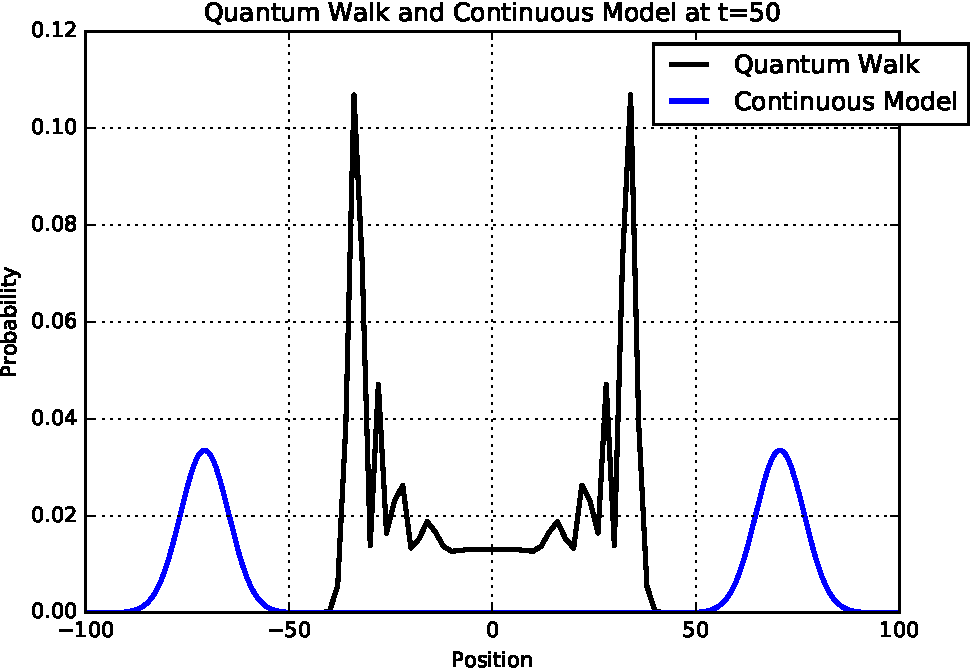
\includegraphics[width=.5\linewidth]{goldwateressay_fig2}
\caption{\footnotesize{A comparison between the probability mass function of the discrete 
Hadamard QRW and probability density function $u$ (solution to the continuous model 
\eqref{classical}) at time $t=50$. Note that the peaks of the continuous model in 
\eqref{classical} and the QRW do not match. Indeed the peaks in case of 
\eqref{classical} spread out much faster than the discrete Hadamard QRW.}}
\label{regplot}
\end{figure}
%
%The PDE in \eqref{classical} is also the limit of a classical random walk without time delays. 
Here we are comparing the probability mass function of discrete Hadamard QRW with a solution to 
\eqref{classical}. 
%The model in \eqref{classical} should capture the diffusive nature of the walk, which is what we are interested in. 
%In Figure \ref{regplot}, the model from Blanchard et.\ al.\ \cite{blanchard} is compared to the probability mass function of the QRW. 
We observe something rather remarkable, we notice that the dynamics of the PDE model 
\eqref{classical} which are labeled as ``Continuous Model" in Figure~\ref{regplot}
spreads out much faster than the dynamics of the discrete Hadamard QRW which are 
labeled as ``Quantum Walk" in Figure~\ref{regplot}. Toward this end we conjecture that 
such a behavior is due to the ``negligence" of waiting time-delays between the jumps while 
deriving \eqref{classical} even though it is unclear to us on how to account for such time-delays 
in the derivation as given in \cite{blanchard}. This will be rigorously justified using 
another an equivalent derivation of \eqref{classical} starting from a generalized-classical
random walk below. 


We next discuss a second approach to derive the PDE system \eqref{classical}, this has been
taken from \cite{barkai}. This approach will further serve as a rigorous motivation for the 
introduction of fractional time derivative. We start with a generalized-classical random
walk on a line. The probability of a walker being at position $y$ at time $s$ is given by:
%
\begin{equation}\label{classical_walk}
p(y,s) = R(y-h)p(y-h,s-\tau)+L(y+h)p(y-h,s-\tau)
\end{equation}
%
where $h,\tau$ are the spatial and time steps, $R$ and $L$ are the probabilities of the walker 
jumping to either right or left. In case of \eqref{classical}, $R(y)-L(y)=\tanh(y)$. Letting  
$R(y)+L(y)=1$ yields $R(y) = \frac{1+\tanh(y)}{2}$ and $L(y) = \frac{1-\tanh(y)}{2}$. By applying
appropriate Taylor expansion to \eqref{classical_walk}, and by taking the limit as $h,\tau\to0$ 
one arrives at \eqref{classical}, we refer \cite{barkai} for details. 



Clearly the derivation of \eqref{classical} using the generalized-random walk does not account for
jump-delays and as a result we arrive at the standard time derivative. We further recall from 
our experiment in Figure~\ref{regplot} that the dynamics of \eqref{classical} needs to be slowed
down in order to match the dynamics of discrete Hadamard QRW. With this goal in mind we recall 
from section~\ref{Brief Introduction to Fractional Calculus} that the a time-delays in a random
leads to (limiting system) the fractional time derivative of order $\alpha \in (0,1)$. 



Our point of departure is the generalized-classical random walk \eqref{classical_walk}.  
By introducing the time-delays, subsequently fractional time derivative in the limit, 
we can approximate the discrete Hadamard QRW better. 
This is quite natural because a fractional time derivative is associated with time delays in the 
random walk.
\LB{The time delays are described by a probability distribution that behaves like \todo{double check what the time delay actually is}{$\mathcal{O}(d^{-(1+\alpha)})$} for large time delays, denoted $d$.
%\begin{equation}
%\frac{\alpha A_\alpha}{\Gamma(1-\alpha)\tau^{(1+\alpha)}}
%\end{equation}
%for large $\tau$ where $\tau$ is \todo{what is $\tau$?}. Moreover $\Gamma(\cdot)$ denotes the 
%standard Gamma function and $A_\alpha$ is a normalization constant that depends on $\alpha$ and the minimum waiting time such that the \HA{probability} distribution integrates to 1. 
%As seen in \cite[Eq.\ 18]{barkai}, $A_\alpha$ acts like the characteristic time step, $\tau$, in the random walk where there is no extra waiting between jumps.
By introducing time delays, }the following fractional PDE can be derived from the generalized-classical random walk \eqref{classical_walk}:
%
\begin{align}\label{fracmodel}
\begin{aligned}
\partial^{\alpha}_{s}u 
 &=\frac{\partial^2}{\partial y^2}u-\frac{\partial}{\partial y}\left[\tanh(y)u\right] 
     \quad \text{in }  (0,\infty)\times\mathbb{R} \\
u(0,y) &=\delta(y), \quad y \in \mathbb{R} \\
\lim_{y\to\pm\infty} u(s,y)&=0, \quad s \in (0,\infty).
\end{aligned}
\end{align}
We refer to \cite[Sec.\ 3]{barkai} for a derivation of the time fractional Fokker Planck 
equation from random walks with time-delays. The same process has been applied to 
\eqref{fracmodel}. The main difference between \eqref{fracmodel} and \eqref{classical} 
is the Caputo fractional time derivative $\partial_t^\alpha$ of order $\alpha \in (0,1)$. 
We refer to \eqref{fracdef} for the definition of $\partial_t^\alpha$. We also recall that
when $\alpha = 1$ then $\partial_s^\alpha = \partial_s$, i.e., \eqref{classical} is a 
special case of our fractional model \eqref{fracmodel}.  
%except the first derivative in time has been replaced by the Caputo fractional derivative, denoted $\partial^{\alpha}_{t}u(t,x)$. The Caputo fractional derivative in time is defined in \eqref{fracdef} for $0<\alpha<1$.
Due to the fact that fractional time derivative is associated to time-delays we expect 
a better match between the solution to \eqref{fracmodel} and discrete Hadamard QRW. 


%Since the fractional time derivative corresponds to classical random walks with time delays, 
%we expect a better match between the fractional model and the QRW. This is our motivation for 
%studying the fractional model in \eqref{fracmodel} instead of \eqref{classical}. An added benefit 
%is that \eqref{classical} is a special case of \eqref{fracmodel}.
% By applying the Riemann Liouville derivative to both sides of \cite[Eq.\ 21]{barkai}, and using the fact that $\prescript{}{0}{D}_t^\alpha f(t) = \frac{f(0)}{t^\alpha\Gamma(\alpha)}+\partial_t^\alpha f(t)$ for absolutely continuous $f$ \cite[Lemma 2.2]{samko_1993}, we arrive at \eqref{fracmodel} for $u$ that is absolutely continuous in $t$. Although we are note guaranteed that $u$ is absolutely continuous in $t$, we argue that modeling with the Caputo derivative is superior for this application because applying initial conditions for the Caputo derivative is much more nature than the Riemann Liouville derivative.  \par





\section{Solving The Fractional Model} \label{s:Solving The Fractional Model} 
To numerically solve the PDE in \eqref{fracmodel}, \LB{we consider the problem
\begin{align}\label{bounded_problem}
\begin{aligned}
\partial^{\alpha}_{t}u 
 &=\frac{\partial^2}{\partial x^2}u-\frac{\partial}{\partial x}\left[\tanh(x)u\right] 
     \quad \text{in }  (0,T)\times\left(-\frac{L}{2},\frac{L}{2}\right) \\
u(0,x) &=\delta(x), \quad x \in \left(-\frac{L}{2},\frac{L}{2}\right) \\
u(t,\pm L/2) &= 0, \quad t\in(0,T).
\end{aligned}
\end{align}
 Here, the problem in \eqref{bounded_problem} is the same as \eqref{fracmodel} except with a bounded domain $(0,T)\times\Omega=(0,T)\times(-\frac{L}{2},\frac{L}{2})$. The value}
  $T>0$ denotes the final time and $L$ denotes the length of the spatial interval. 
\LB{Because we are working on a finite interval, we need to impose boundary conditions on the PDE. We choose homogeneous Dirichlet boundary conditions at $x=\pm\frac{L}{2}$, i.e. $u\left(t,\pm \frac{L}{2}\right) = 0$. Since $\lim_{x\to\infty}u(t,x) = 0$ in \eqref{fracmodel}, using homogenous Dirichlet boundary conditions with $L$ large will approximate the original boundary conditions in \eqref{fracmodel} well.}

\LB{In order to numerically solve \eqref{bounded_problem}, we break up the scheme into a few steps. First, we approximate the initial conditions the the PDE. Next, we use a spectral method for the spatial discretization and use a finite difference scheme for the discretization in time.}
%Instead of the boundary conditions in the limit in \eqref{fracmodel}, we set homogeneous Dirichlet boundary conditions at $x=\pm\frac{L}{2}$.

For the initial condition, we use a Dirac sequence to approximate the Dirac delta function.
A Dirac sequence $\delta_n(x)$ satisfy the following two properties \cite[Sec. 8.7]{arfken_1985}:
\begin{align}
&\int_{-\infty}^{\infty}\delta_n(x)\,\mathrm{d}x=1, \text{ for all } n\in\mathbb{N}\nonumber\\
\lim_{n\to\infty}&\int_{-\infty}^{\infty}\delta_n(x)f(x)\,\mathrm{d}x = f(0). \label{dirac_sequence_properties}
\end{align}
The initial condition is then defined as
$$\delta(x)=\lim_{n\to\infty}\delta_n(x).$$

Taking $n$ large will approximate the Dirac delta initial condition. We let $\delta_n(x)$ to be 
\begin{equation}\label{dirac_sequence}
\delta_n(x) = \begin{cases}
0,& x\leq\frac{2}{n}\\
\frac{2n}{3} + \frac{n^2}{3}x,& -\frac{2}{n}<x\leq-\frac{1}{n}\\
\frac{n}{3},& \frac{-1}{n}<x\leq\frac{1}{n}\\
\frac{2n}{3} - \frac{n^2}{3}x,& \frac{1}{n}<x\leq\frac{2}{n}\\
0,& \frac{2}{n}<x.\\
\end{cases}
\end{equation}
\LB{Figure \ref{dirac_sequence_fig} gives three $\delta_n(x)$ from our Dirac Sequence\eqref{dirac_sequence}.
By Lemma \ref{integral_lemma} and Theorem \ref{dirac_theorem} in Appendix \ref{s:dirac_sequence_proof}, this choice of approximation satisfies the desired properties in \eqref{dirac_sequence_properties}. An additional property is that our Dirac sequence is piecewise linear, which means that the trapezoid rule for numerical quadrature will be exact for a small enough spatial mesh. Finally, given a spatial mesh size of $h$, we choose $n$ so that $\frac{1}{n}>h$, which means a piecewise linear interpolation can represent the initial condition approximation exactly.}

\begin{figure}[h!]
\begin{center}\label{dirac_sequence_fig}
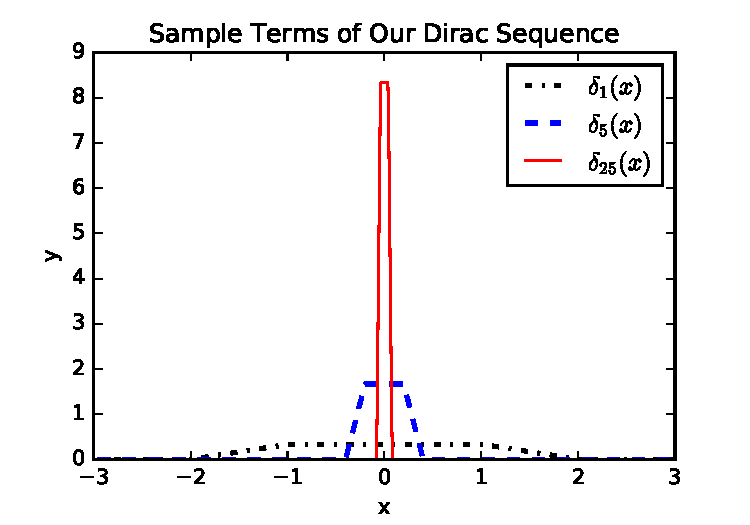
\includegraphics[width=.5\textwidth]{delta_sequence}
\caption{Dirac sequence from \eqref{dirac_sequence}}
\end{center}
\end{figure}


\LB{For the spatial discretization, we utilize a spectral method. In particular, we use the sine transform the incorporate the homogenous Dirichlet boundary conditions. By taking the sine transform} with respect to the spatial variable $x$, \eqref{fracmodel} becomes
\begin{equation}
\partial^{\alpha}_{t}\mathcal{F}_s\{u\}=-\frac{\pi^2\omega^2}{2L^2}\mathcal{F}_s\{u\}+\frac{\pi\omega}{L}\mathcal{F}_c\{\tanh(x)u\},\label{sineq}
\end{equation}
where $\mathcal{F}_s\{u\}$ is the sine transform of $u$, $\omega$ is the frequency variable, and \LB{$\mathcal{F}_c\{\tanh(x)u\}$ is the cosine transform of $\tanh(x)u$. Note that $\frac{\pi\omega}{L}\mathcal{F}_c\{\tanh(x)u\} = \mathcal{F}_c\{\frac{\partial}{\partial x}[\tanh(x)u]\}.$}

\LB{For the discretization in time, we use a finite difference scheme.} We specifically use a $L1$ approximation scheme to approximate $\partial_{t}^{\alpha}u$ with time values $t_k=k\tau$ for $k\in\mathbb{N}$ and time step $\tau$ (c.f.\ \cite{lin}). The discretization is achieved by taking a backward difference approximation for $u_t$ in \eqref{fracdef}. The resulting discretization for $\partial_{t}^{\alpha}u(t_{k+1},x)$ is
\begin{align}
\partial_{t}^{\alpha}u(t_{k+1},x)&\approx\frac{1}{\Gamma(1-\alpha)}\sum_{\ell=0}^{k}\int_{t_{\ell}}^{t_{\ell+1}}\frac{[u(t_{\ell+1},x)-u(t_\ell,x)]/\tau}{(t_{k+1}-y)^{\alpha}}dy \nonumber\\
&=\frac{1}{\Gamma(2-\alpha)}\sum_{\ell=0}^{k}\frac{u(t_{\ell+1},x)-u(t_\ell,x)}{\tau^\alpha}a_{k-\ell}\label{discretization}
\end{align}
where $a_{k-\ell}=(k+1-\ell)^{1-\alpha}-(k-\ell)^{1-\alpha}$.

\LB{To attain a solution to our PDE, we apply the $L1$ scheme to the sine transformed PDE to produce an iterative scheme. Applying the $L1$ scheme to the left hand side of \eqref{sineq},} we get 
\begin{equation}
\frac{1}{\Gamma(2-\alpha)}\sum_{\ell=0}^{k}\frac{\hat{u}_{\ell+1}-\hat{u}_{\ell}}{\tau^\alpha}a_{k-\ell}=-\frac{\pi^2\omega^2}{2L^2}\hat{u}_{k+1}+\frac{\pi\omega}{L}\mathcal{F}_c\{\tanh(x)u_{k+1}\}\label{freqdiscrete}
\end{equation}
where $\hat{u}_{k}$ denotes the sine transform of $u$ at time step $t_k$. By isolating $\hat{u}_{k+1}$ in \eqref{freqdiscrete}, we arrive at the following equation
\begin{equation}
\hat{u}_{k+1}=C_2\left[\frac{\pi\omega}{L}\mathcal{F}_c\{\tanh(x)u_{k+1}\}+C_1\left(\hat{u}_k-\sum_{\ell=0}^{k-1}(\hat{u}_{\ell+1}-\hat{u}_{\ell})a_{k-\ell}\right)\right]
\end{equation}
where $C_1=\left(\Gamma(2-\alpha)\tau^\alpha\right)^{-1}$ and $C_2=\left(C_1+\frac{\pi^2\omega^2}{2L^2}\right)^{-1}$.

\LB{Since $\mathcal{F}_c\{\tanh(x)u_{k+1}\}$ is on the right hand side, we use} a fixed point iteration is then used to solve for $u_{k+1}$ at every time iteration. Algorithm \ref{FPIalgorithm} implements the nested fixed point iteration and give us the numerical solution to \eqref{bounded_problem}. The outer iteration is the time evolution while the inner iteration is the fixed point iteration.
\begin{algorithm}[h!]\begin{algorithmic}[1]
\STATE{$C_1\leftarrow\left(\Gamma(2-\alpha)\tau^\alpha\right)^{-1}$}
\STATE{ $C_2\leftarrow\left(C_1+\frac{\pi^2\omega^2}{2L^2}\right)^{-1}$}
\FOR{$k=\{1,\ldots, K\}$}
\STATE $u_{k+1,\ 0}\leftarrow u_{k}$
\WHILE{$|u_{k+1,\ j+1}-u_{k+1,\ j}|/|u_{k+1,\ j}|>\epsilon$}
\STATE $\hat{f}_{k+1,\ j}\leftarrow\frac{\pi\omega}{L}\mathcal{F}_c\{\tanh(x)u_{k,\ j}\}$
\STATE $\hat{u}_{k+1,\ j+1}\leftarrow C_2\left[\hat{f}_{k+1,\ j}+C_1\left(\hat{u}_k-\sum_{\ell=0}^{k-1}(\hat{u}_{\ell+1}-\hat{u}_{\ell})a_{k-\ell}\right)\right]$
\STATE $u_{k+1,\ j+1}\leftarrow\mathcal{F}^{-1}_s\{\hat{u}_{k+1,\ j+1}\}$
\ENDWHILE
\STATE $u_{k+1} \leftarrow u_{k+1,\ j+1}$
\ENDFOR
\RETURN $\{ u_1,\ldots,u_K\}$
\end{algorithmic}
\caption{Nested FPI }
\label{FPIalgorithm}
\end{algorithm}
\section{Convergence of Numerical Scheme} \label{s:Convergence}
The authors in \cite{blanchard} provide an analytical solution to 
\LB{\eqref{classical}, which is a special case of our model with $\alpha=1$. We know the analytical solution for \eqref{classical}, so we conduct numerical experiments to check for the rate of convergence of the method. This is not a proof of convergence but provides a ceh that our computations are producing reasonable results.} 
To test for convergence, we solved the PDE in \eqref{classical} on the domain $\Omega=(0,10)\times(-200,200)$. For the rate of convergence in time, we refine the mesh in time and compute the $L^2$ error while holding the spatial mesh size constant. Likewise for the spatial rate of convergence, we refine the mesh in space and compute the $L^2$ error while holding the time mesh size constant.
\begin{figure}[h!] %fix the L^2 stuff
\begin{center}
\begin{minipage}{.5\textwidth}
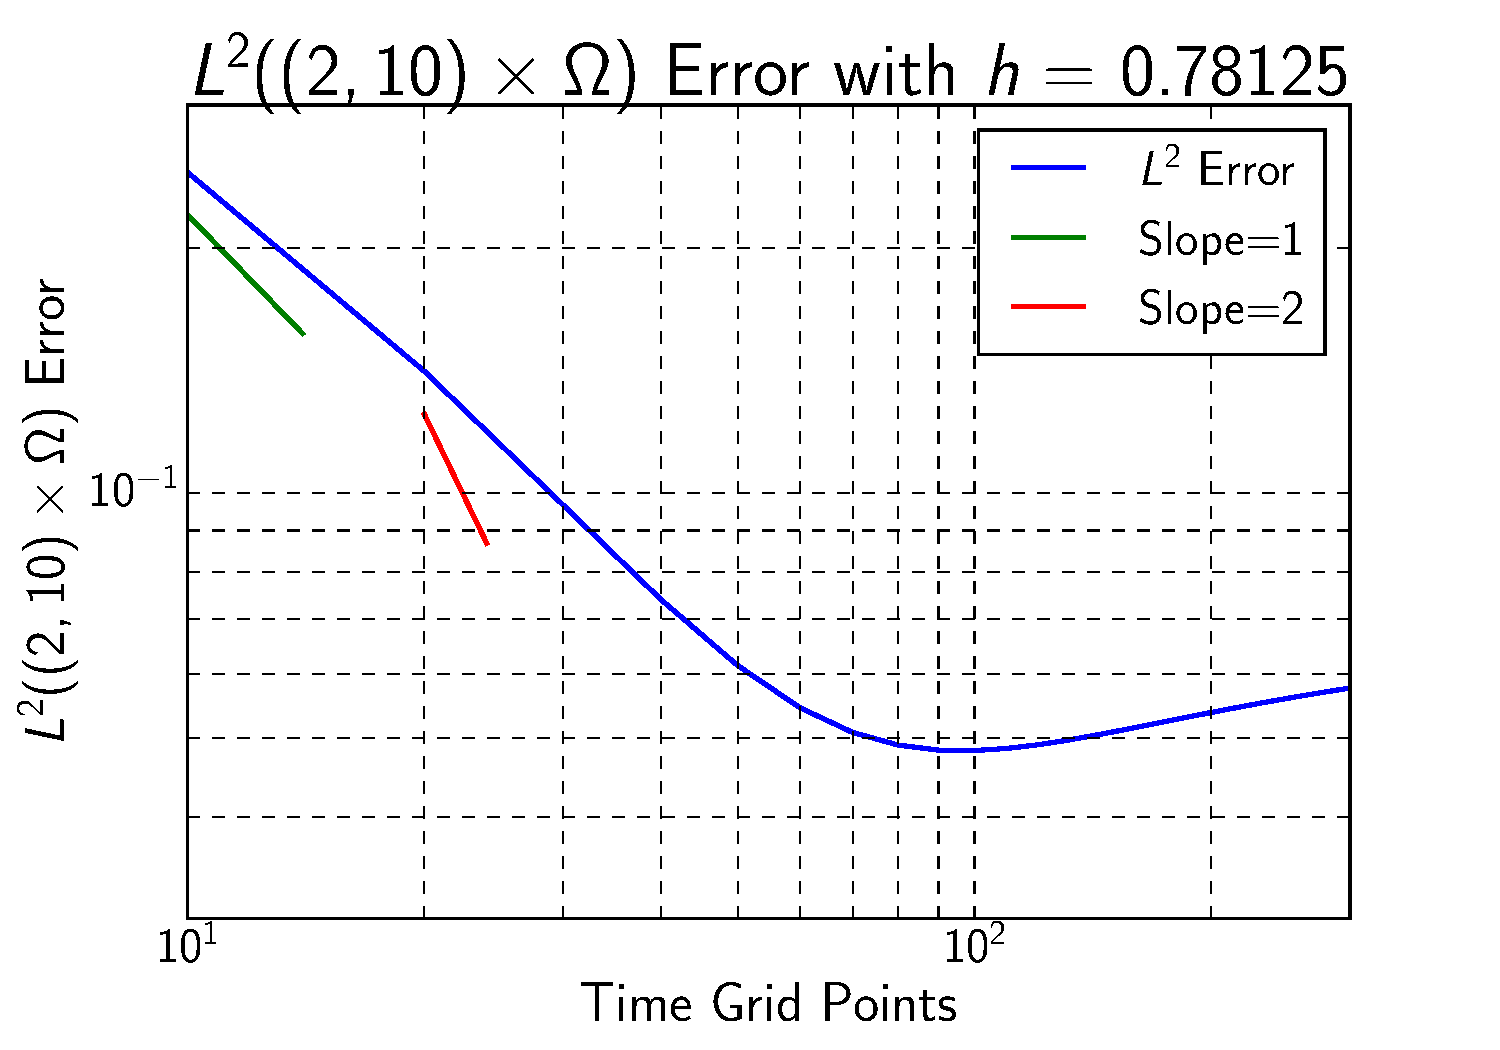
\includegraphics[width=\linewidth]{L2_timeErr2}
\end{minipage}%
\begin{minipage}{.5\textwidth}
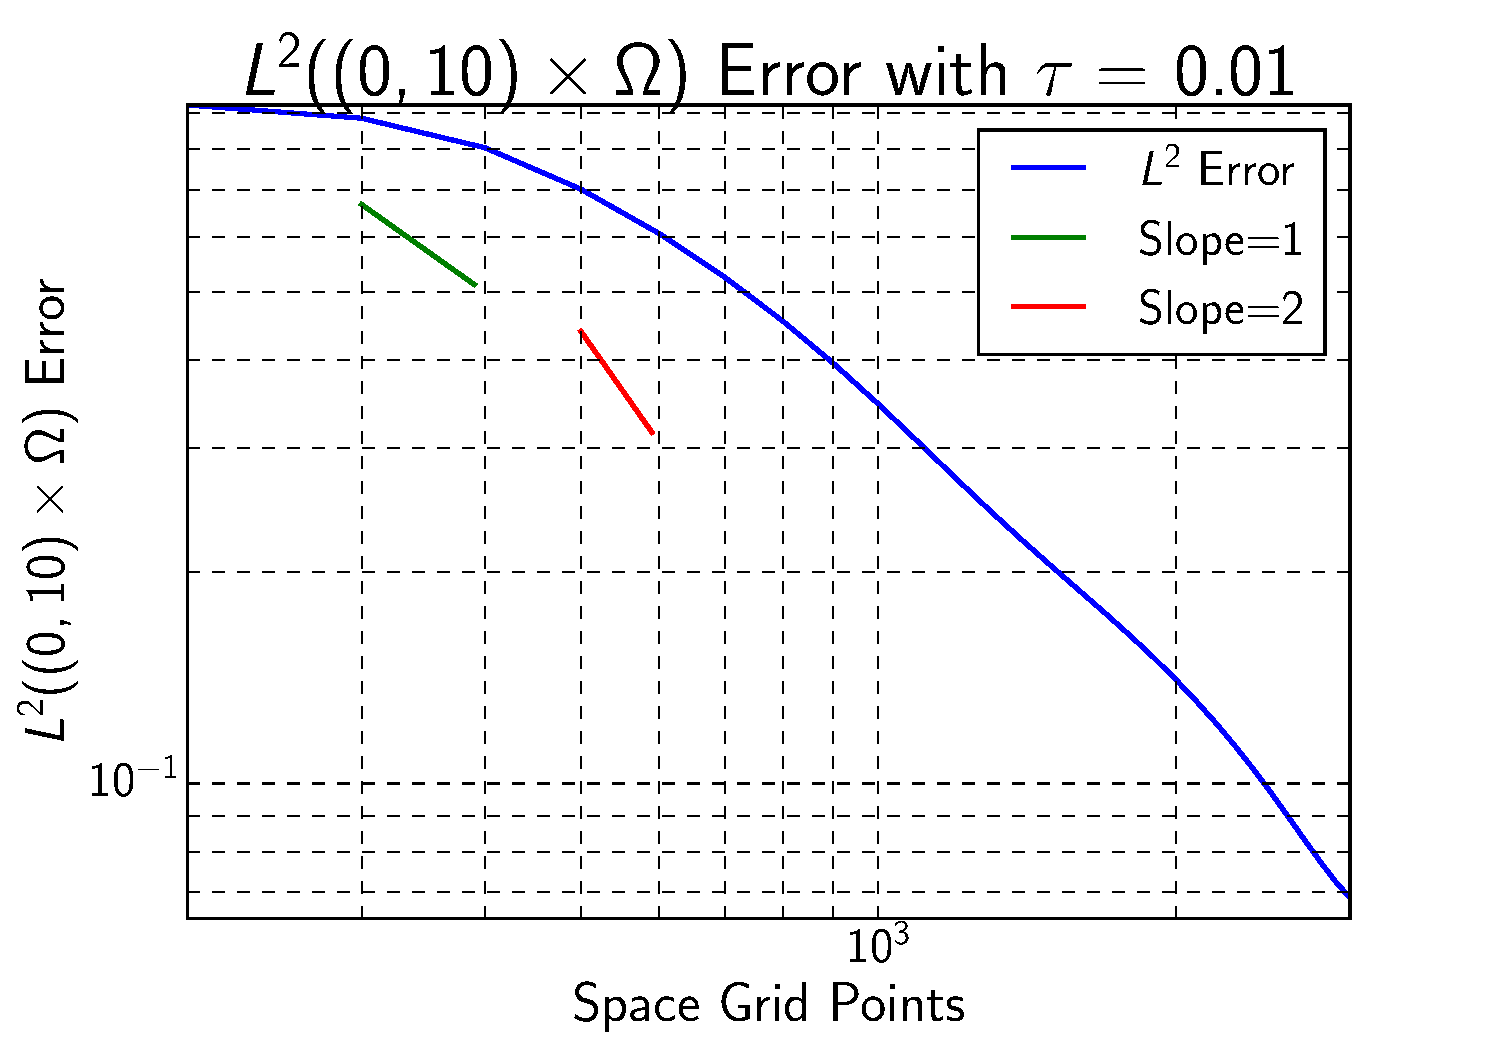
\includegraphics[width=\linewidth]{L2_spaceErr1}
\end{minipage}%
\end{center}
\label{errorplot}
\caption{{\footnotesize The left figure is the $L^2$ norm on the subdomain $(2,10)\times\Omega$ with respect to time refinements and the right figure is the $L^2$ norm on the subdomain $(0,10)\times\Omega$ with respect to space refinements. We can see that the $L^2$ error converges at a rate approximately 1 with respect to time and space refinements.}}
\end{figure}
\LB{
Figure \ref{errorplot} demonstrates the convergence with respect to time refinements on the subdomain $(2,10)\times(-200,200)$. The subdomain $(2,10)\times(-200,200)$ is shown because the method does not seem to converge on the whole domain $(0,10)\times(-200,200)$. This is due to the irregularity of the initial condition, which hurts the convergence of the method close to the initial time. On the subdomian $(2,10)\times(-200,200)$, the rate of convergence is approximately 1. This is consistent with the fact that the $L1$ scheme is the same as the Backward Euler scheme for $\alpha = 1$.}
\LB{
Figure \ref{errorplot} demonstrates the convergence with respect to space refinements on $(0,10)\times(-200,200)$.The method is approximately first order with respect to spatial refinements. Spectral methods usually exhibit a high rate of convergence, but the irregular initial conditions cause the lower rate of convergence in our case.}

\LB{The numerical experiment discussed was for $\alpha=1$. For values of $\alpha$ other than 1, the regularity of the solution to \eqref{fracmodel} may be worse, which will give a slower rate of convergence. For example, the time fractional heat equation, $\partial^\alpha_tu = u_{xx}$, can have solutions with that are not continuously differentiable with respect to time \cite{stynes}. The Dirac delta initial condition further While an error analysis of the $L1$ scheme for the time fractional heat equation exists for initial conditions that are $L^2(\Omega)$ \cite{jin}, more work must be done on error estimates for initial conditions not in $L^2(\Omega)$, like in our case.}

\section{Optimization Method to Calculate $\alpha$} \label{s:Optimization}
Figure~\ref{cumulativeplot} depicts cumulative probability distributions for the QRW, the model from \cite{blanchard}, and our fractional model. For the QRW, we calculate the cumulative probabilities by summing up individual probabilities up to the specific spatial value in the plot. For the two continuous models, the cumulative probability is calculated using a trapezoid method. As seen in Figure~\ref{cumulativeplot}, the fractional model with $\alpha=.75$ provides a much more accurate depiction of the QRW and is a significant improvement over the model in \cite{blanchard}.
\begin{figure}[h!]
\centering
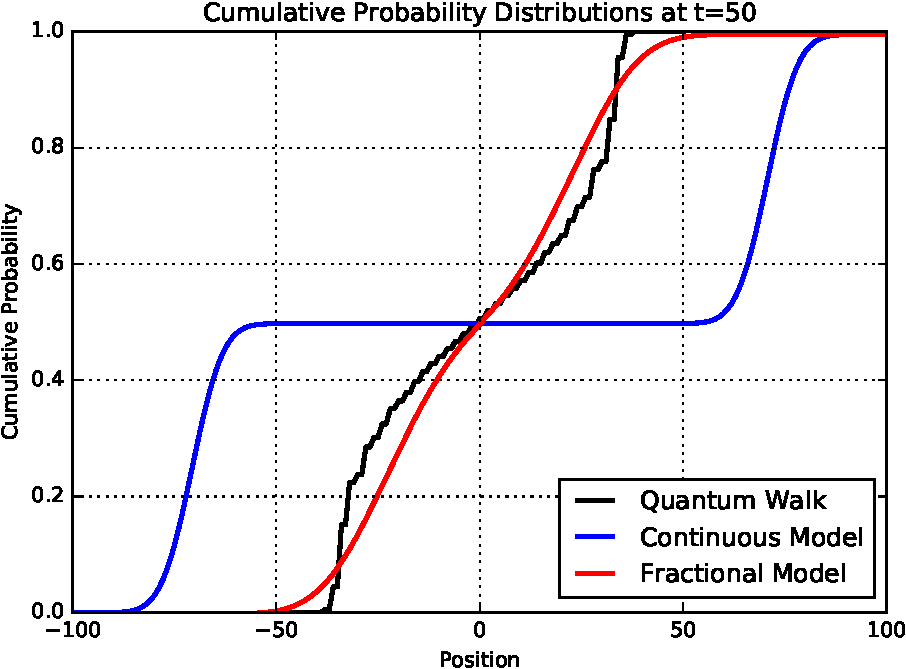
\includegraphics[width=.5\linewidth]{goldwateressay_fig1}
\caption{\footnotesize{Cumulative Probability Distributions of the QRW, regular model from \cite{blanchard}, and the fractional model with $\alpha=.75$.}}
\label{cumulativeplot}
\end{figure}
%One observation from Figure~\ref{cumulativeplot} is that the peaks in the fractional model do not spread as quickly as the model in \cite{blanchard}. 
The choice of $\alpha=.75$ was arbitrary. We'll devote the next section to the optimization algorithm that will determine the best choice for $\alpha$.


As mentioned previously, there was a large discrepancy between the continuous model from  \cite{blanchard} and the QRW (c.f.\ Figure \ref{cumulativeplot}). Our original motivation for introducing the fractional derivative was to overcome this discrepancy. We have now introduced the fractional model and have seen the improved fit for when $\alpha=.75$, but the choice of $\alpha$ was arbitrary. One way to decide $\alpha$ would be to optimize for the fit of the QRW with respect to $\alpha$. By choosing the optimal $\alpha$, we will have a much clearer picture of how exactly the fractional model fits the QRW. The approach we will use has been previously utilized for finding the optimal order of the fractional Laplacian in \cite{valdinoci_opt}.

\LB{We want to find the optimal $\alpha$ such that we have the best fit between the QRW and the fractional PDE model. The Hadamard QRW is discrete in space and our PDE model is continuous in space, so the notion of best fit should be the best fit between cumulative distributions. Another aspect to consider is the domain of definition for $\alpha$. The fractional model in \eqref{fracmodel} assumes that $0<\alpha<1$. To make sure that an optimization process stays within $0<\alpha<1$, we add an additional term to the functional we will be minimizing. This additional term will be convex and have asymptotes at $\alpha=0$ and $\alpha = 1$ to ensure that an optimization process stays within $0<\alpha<1$. The resulting} functional we will be minimizing is 
\begin{equation}\label{objectivefunctional}
J[\alpha] = \frac{1}{2}\int_0^T\int_{\Omega}(u_\alpha-q)^2\, \mathrm{d}x\mathrm{d}t+\gamma\frac{1}{(1-\alpha)\alpha}
\end{equation}
where $u_\alpha$ is the cumulative probability distribution of the solution to our fractional PDE model with the derivative order $\alpha$ and $q$ is the linear interpolant of the QRW cumulative probability distribution. The far right term will prevent the optimization process from going outside the interval $(0,1)$, with $0<\gamma<<1$. This will ensure that our optimization stays inside the domain of definition for the fractional PDE model. With a small $\gamma$ our optimization will be most influenced by the first term, which measures how good the fit of $u_\alpha$ is to $q$. 

\LB{To minimize the functional in \eqref{objectivefunctional}, we employ a gradient descent method. In order to use the gradient descent, we need an approximation for the gradient of $J$.} Using a right hand Riemann sum approximation with space and time step sizes $h,\tau$ for the integral, the approximation of the gradient for \eqref{objectivefunctional} is
\begin{equation}\label{functionalgradient}
J'[\alpha] = h\tau\sum_{i}\sum_{j}\left[(u_\alpha(t_i,x_j)-q(t_i,x_j))\frac{d}{d\alpha}u_\alpha(t_i,x_j)\right]+\gamma\frac{2\alpha-1}{(1-\alpha)^2\alpha^2},
\end{equation}
where $\frac{d}{d\alpha}u_\alpha(t_i,x_j)$ denotes a backwards difference approximation of the derivative of $u_\alpha(t_i,x_j)$ with respect to $\alpha$. The resulting gradient descent algorithm in Algorithm \ref{gradientdescent} \LB{is how we minimize} the functional in \eqref{objectivefunctional}.
\begin{algorithm}[H]
\begin{algorithmic}[1]
%\Function{gradientDescent}{tol,$\lambda$,$\alpha$} 
\STATE set tolerance tol
\STATE initialize $\lambda$
\STATE initialize an initial guess$\alpha$
\STATE compute $J'[\alpha]$
\WHILE{$|J'[\alpha]|>\text{tol}$}
\STATE $\alpha \leftarrow \alpha-\lambda J'[\alpha]$
\STATE compute new $J'[\alpha]$
\ENDWHILE
\RETURN $\alpha$
% \EndFunction
\end{algorithmic}
\caption{Gradient Descent }
\label{gradientdescent}
\end{algorithm}

Another key addition to Algorithm \ref{gradientdescent}, is to conduct two passes of the gradient descent. The first pass will be on a coarse mesh, specifically $h,\tau=.2$ and $\lambda=1$. The optimal $\alpha$ from this first pass \LB{will give us a good initial guess for the optimal $\alpha$ for the second pass. The second pass} will be on a finer mesh, specifically $h,\tau=.1$ and $\lambda=.5$. Additionally, the tolerance is set to be $10^{-4}$. 
%If the tolerance is smaller, $\frac{d}{d\alpha}u_\alpha(t_i,x_j)$ becomes unstable.

\section{Optimization Results} \label{s:Optimization Results}
After applying the prescribed optimization routine for different values for $T$, the following table lists the corresponding optimal $\alpha$ values.
\begin{table}[h!]
\centering
\begin{tabular}{ |c | c | c | c | c |c |c |c |c |c |c |c |c}
\hline
T 			   & 10 	& 20 		& 30 		& 40 		& 50 		& 60 		& 70 	 	& 80		& 90 \\\hline
Optimal $\alpha$ & 0.645 & 0.701 	& 0.724 	& 0.742 	& 0.754 	& 0.763	& 0.771 	& .776	& .781 \\\hline
\end{tabular}
\caption {Optimal $\alpha$ values at differing $T$ values}
\label{optimizationresults}
\end{table}

One observation from Table \ref{optimizationresults} is that our original guess of $\alpha=.75$ was relatively accurate. Another observation is that $\alpha$ is increasing for increasing $T$. 
%This seems to be consistent with the model from \cite{blanchard} due to the author's from \cite{blanchard} noting that their model is a better fit as $T\to\infty$. 
\begin{figure}[h!]
\centering
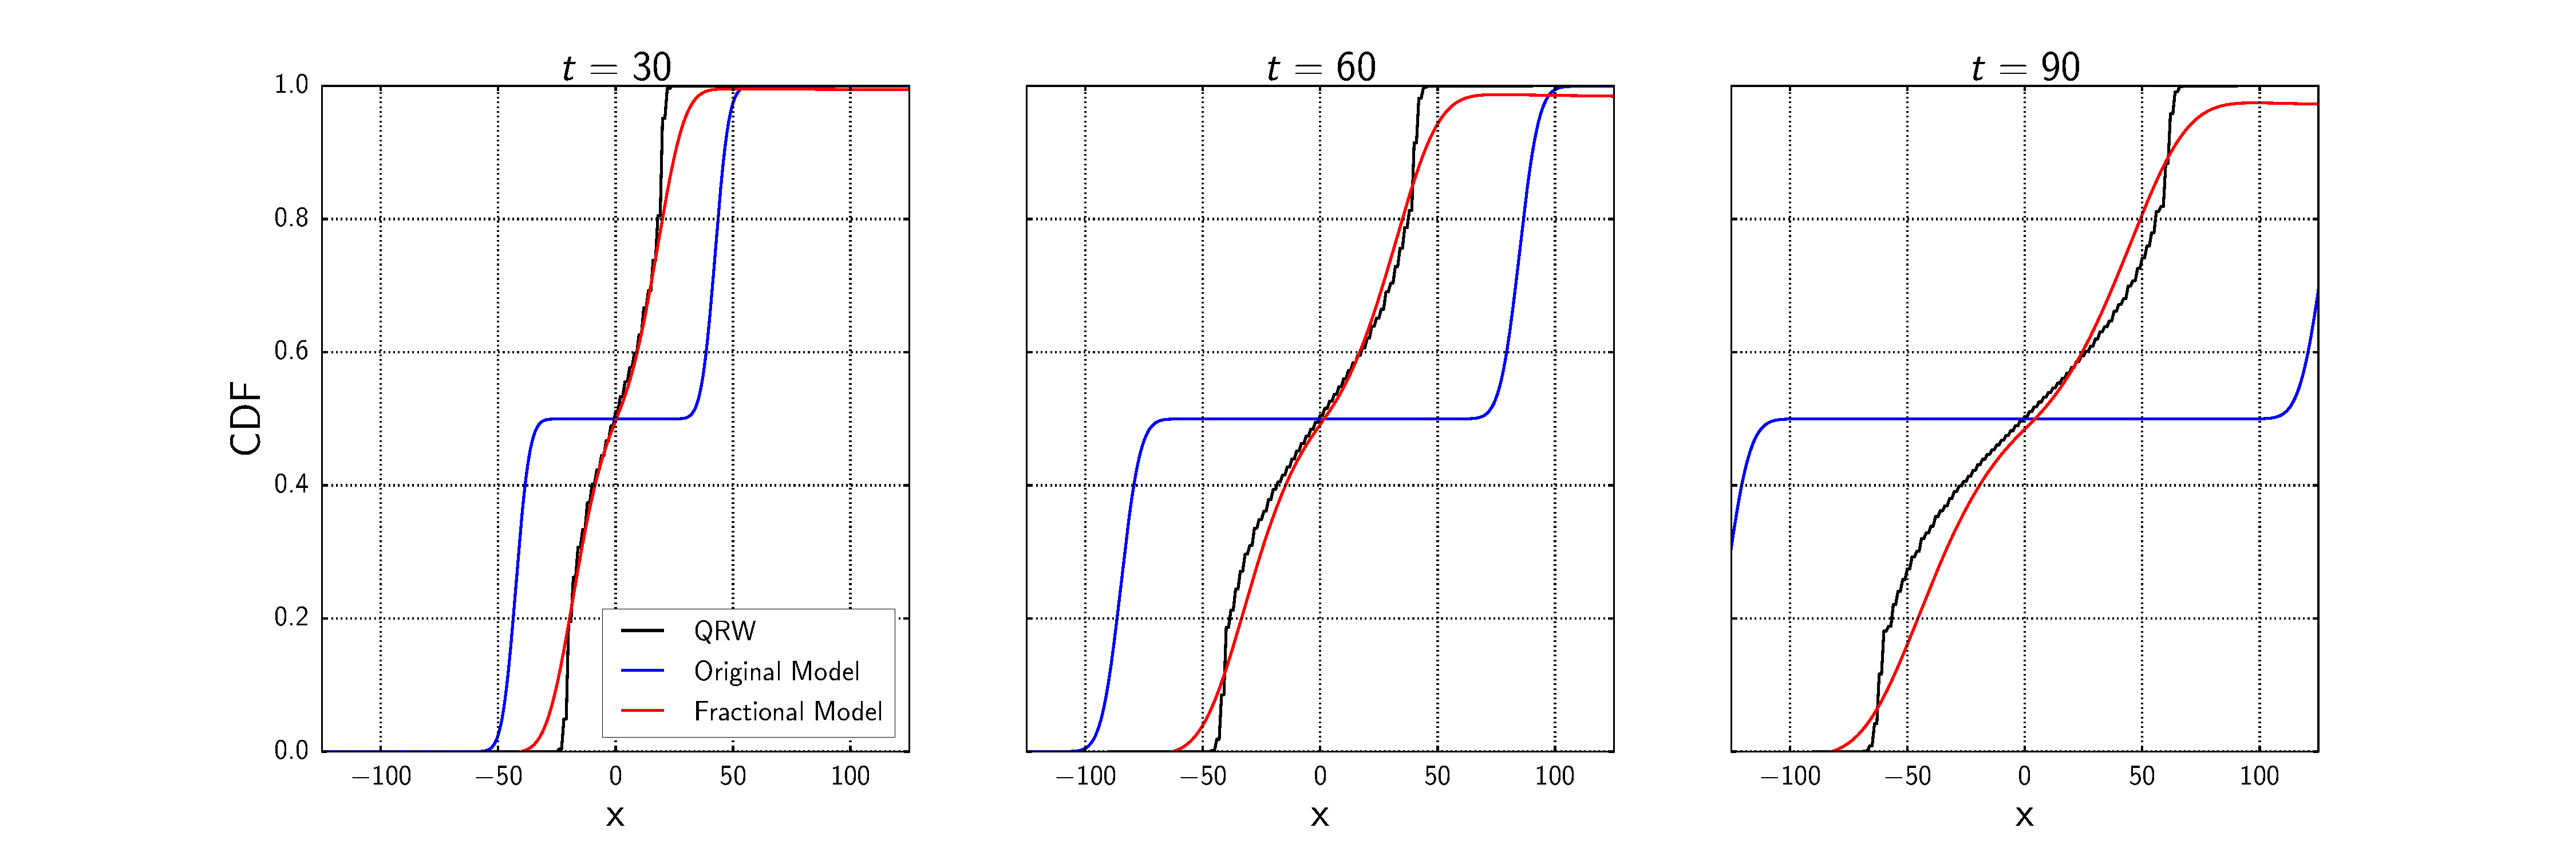
\includegraphics[clip, trim=6.5cm .5cm 6.5cm 1.50cm, width=1.00\textwidth]{opt5_90results}
\caption{Comparison of CDFs from the QRW and the fractional model with the optimal $\alpha$ value from when $T=90$}
\label{resultsT90}
\end{figure}
Figure \ref{resultsT90} depicts the fractional model with $\alpha=.781$ compared to the QRW at different time values. We can see that the optimization algorithm has provided a value for $\alpha$ that matches the QRW closely, which is an improvement over the previous model.


\section{Conclusions and Future Work} \label{s:Conclusion}\todo{write more in conclusion and recall to reader why they should care}
To summarize, we first noted a large discrepancy between the discrete QRW and the continuous model from \cite{blanchard}. To enrich the model from \cite{blanchard}, we introduced a fractional derivative in time. We provided a numerical method to approximate the solution to the fractional model and provided an optimization algorithm to choose the order of the fractional derivative that would best fit the discrete QRW. Our results show that the introduced fractional model is a an improvement over the previous continuous model in the literature. As a result, we have introduced the first continuous model that can model discrete QRW dynamics effectively. Future work involves an analysis of the numerical scheme for the fractional problem and analysis of the optimization problem and the numerical scheme to solve it.

\section*{Acknowledgments}
We would like to thank Marco Lanzagorta for introducing us to the topic of Quantum Random Walks. We would also like to thank Salvador Venegas-Andraca for providing us helpful comments and feedback on this paper.


\appendix
\section{Proof that our Dirac Sequence in \eqref{dirac_sequence} Satisfies the Properties in \eqref{dirac_sequence_properties}}\label{s:dirac_sequence_proof}
For our Dirac sequence in \eqref{dirac_sequence} to satisfy the properties in \eqref{dirac_sequence_properties}, we need every element of the sequence to integrate to 1. In the limit, we want the Dirac sequence integrated against a continuous function $f$ to concentrate the integral on the value $f(0)$. The first Lemma gives us the first condition.
\begin{lemma} \label{integral_lemma}
Let $\delta_n$ be defined as in \eqref{dirac_sequence}. Then,
$$\int_{-\infty}^{\infty}\delta_n(x)\mathrm{d}x=1.$$
\end{lemma}
\begin{proof}
Every element of the sequence is a trapezoid with base lengths $\frac{4}{n},\frac{2}{n}$ and height $\frac{n}{3}$. The area of this trapezoid is 1 for all $n$. 
%Let our Dirac sequence be defined by \eqref{dirac_sequence}. Because $\delta_n(x)=0$ for $|x|>\frac{2}{n}$,
%$$\int_{-\infty}^{\infty}\delta_n(x)\mathrm{d}x = \int_{-\frac{2}{n}}^{\frac{2}{n}}\delta_n(x)\mathrm{d}x.$$
%Using the piecewise definition of $\delta_n(x)$, we'll split the integral into separate parts.
%\begin{align}
%\int_{-\frac{2}{n}}^{\frac{2}{n}}\delta_n(x)\mathrm{d}x &= \int_{-\frac{2}{n}}^{\frac{-1}{n}}\delta_n(x)\mathrm{d}x+\int_{-\frac{1}{n}}^{\frac{1}{n}}\delta_n(x)\mathrm{d}x+\int_{\frac{1}{n}}^{\frac{2}{n}}\delta_n(x)\mathrm{d}x\nonumber\\
%&=\int_{-\frac{2}{n}}^{\frac{-1}{n}}\frac{2n}{3}+\frac{n^2}{3}x\mathrm{d}x+\int_{-\frac{1}{n}}^{\frac{1}{n}}\frac{n}{3}\mathrm{d}x+\int_{\frac{1}{n}}^{\frac{2}{n}}\frac{2n}{3}-\frac{n^2}{3}x\mathrm{d}x\nonumber\\
%&=\int_{-\frac{2}{n}}^{\frac{-1}{n}}\frac{2n}{3}+\frac{n^2}{3}x\mathrm{d}x+\frac{2}{3}+\int_{\frac{1}{n}}^{\frac{2}{n}}\frac{2n}{3}-\frac{n^2}{3}x\mathrm{d}x\label{integral_triangles}
%\end{align}
%The other integrals to evaluate in \eqref{integral_triangles} are both the area of a right triangle with height $\frac{n}{3}$ and width $\frac{1}{n}$. The resulting integrals are
%$$\int_{-\frac{2}{n}}^{\frac{-1}{n}}\frac{2n}{3}+\frac{n^2}{3}x\mathrm{d}x+\frac{2}{3}+\int_{\frac{1}{n}}^{\frac{2}{n}}\frac{2n}{3}-\frac{n^2}{3}x\mathrm{d}x = \frac{1}{6}+\frac{2}{3}+\frac{1}{6}=1,$$
%which is what we want.
\end{proof}
The Lemma shows that $\delta_n$ integrates to 1, but it will also be helpful in showing that $\delta_n$ satisfies the next property.
\begin{theorem} \label{dirac_theorem}
Let $f:\mathbb{R}\to\mathbb{R}$ be continuous at $x=0$ and let $\delta_n$ be defined as in \eqref{dirac_sequence}. Then,
$$\lim_{n\to\infty}\int_{-\infty}^{\infty}\delta_n(x)f(x)\mathrm{d}x=f(0).$$
\end{theorem}
\begin{proof}
Let $f:\mathbb{R}\to\mathbb{R}$ be continuous at $x=0$. By Lemma \ref{integral_lemma},
\begin{align*}
\lim_{n\to\infty}\left|\int_{-\infty}^{\infty}\delta_n(x)f(x)\mathrm{d}x-f(0)\right| =& \lim_{n\to\infty}\left|\int_{-\frac{2}{n}}^{\frac{2}{n}}\delta_n(x)(f(x)-f(0))\mathrm{d}x\right|\\
\leq&  \lim_{n\to\infty}\int_{-\frac{2}{n}}^{\frac{2}{n}}\left|\delta_n(x)(f(x)-f(0))\right|\mathrm{d}x.
\end{align*}
%\begin{align}
%\lim_{n\to\infty}\left|\int_{-\infty}^{\infty}\delta_n(x)f(x)\mathrm{d}x-f(0)\right| &= \lim_{n\to\infty}\left|\int_{-\frac{2}{n}}^{\frac{2}{n}}\delta_n(x)f(x)\mathrm{d}x-f(0)\right| \nonumber\\
%&=\lim_{n\to\infty}\left|\int_{-\frac{2}{n}}^{\frac{2}{n}}\delta_n(x)f(x)\mathrm{d}x-f(0)\int_{-\frac{2}{n}}^{\frac{2}{n}}\delta_n(x)\mathrm{d}x\right| \nonumber\\
%&=\lim_{n\to\infty}\left|\int_{-\frac{2}{n}}^{\frac{2}{n}}\delta_n(x)(f(x)-f(0))\mathrm{d}x\right|\label{int_limit}
%\end{align}
By the Cauchy-Schwarz inequality, 
$$\lim_{n\to\infty}\int_{-\frac{2}{n}}^{\frac{2}{n}}\left|\delta_n(x)(f(x)-f(0))\right|\mathrm{d}x\leq \lim_{n\to\infty}\int_{-\frac{2}{n}}^{\frac{2}{n}}\left|f(x)-f(0)\right|\mathrm{d}x\int_{-\frac{2}{n}}^{\frac{2}{n}}\left|\delta_n(x)\right|\mathrm{d}x.$$
By Lemma \ref{integral_lemma}, $\int_{-\frac{2}{n}}^{\frac{2}{n}}\delta_n(x)\mathrm{d}x=1$, so we have
$$\lim_{n\to\infty}\int_{-\frac{2}{n}}^{\frac{2}{n}}\left|f(x)-f(0)\right|\mathrm{d}x\int_{-\frac{2}{n}}^{\frac{2}{n}}\left|\delta_n(x)\right|\mathrm{d}x \leq \lim_{n\to\infty}\frac{4}{n}\max_{|x|\leq\frac{2}{n}}|f(x)-f(0)|$$
Because $f$ is continuous, $\max_{|x|<\frac{2}{n}}|f(x)-f(0)|\to0$ as $n\to\infty$, and 
$$\lim_{n\to\infty}\left|\int_{-\infty}^{\infty}\delta_n(x)f(x)\mathrm{d}x-f(0)\right|=0.$$
\end{proof}




\bibliographystyle{plain}
\bibliography{refs}

\end{document}  